\documentclass[12pt,a4paper]{article}
% 如果需要中文支持，推荐使用xeCJK + 字体设置
% \usepackage{xeCJK}
% \setCJKmainfont{SimSun}  % 示例：宋体，可根据系统字体情况更换
\usepackage{ctex}
\setlength{\parindent}{2em}
\setlength{\parskip}{0pt} % 确保段落之间没有额外的空行间距


\usepackage{amsmath}      % 数学公式（如有需要）
\usepackage{graphicx}     % 插图
\usepackage{geometry}     % 调整页边距
\usepackage{fancyhdr}     % 自定义页眉页脚
\usepackage{indentfirst}  % 中文首行缩进
\usepackage{calc}         % 允许做长度运算(测量文字宽度等)
\usepackage{titlesec}
\usepackage{booktabs} % 解决 \midrule 和 \bottomrule 报错
\usepackage{enumitem} % 支持自定义列表格式
\usepackage{float}    % 支持强制浮动位置

% 设置 \section 级标题为：加粗、大字号（如 \Large）
\titleformat{\section}
	{\bfseries\large}    % 标题自身的格式
	{\thesection}        % 标题编号的显示方式
	{1em}                % 编号与标题文字之间的间距
	{}                   % 在标题文字前后可插入额外代码，此处为空
	
% 设置 \subsection 级标题为：加粗、中等字号（如 \normalsize）
\titleformat{\subsection}
	{\bfseries\normalsize}
	{\thesubsection}
	{1em}
{}

% 页面设置（可根据需要微调）
\geometry{
	left=2cm,
	right=2cm,
	top=1cm,
	bottom=1.5cm
}

% 不需要过大的行距，使用较接近单倍行距的设置
\renewcommand{\baselinestretch}{1.2}

% 仅在页脚居中显示页码，页眉保持为空
\pagestyle{fancy}
\fancyhf{}  % 清空默认的页眉页脚
\fancyfoot[C]{\thepage}
\renewcommand{\headrulewidth}{0pt}
\renewcommand{\footrulewidth}{0pt}

% 首行缩进2字符(中文习惯)
\setlength{\parindent}{0pt}
\setlength{\leftskip}{2em}

\begin{document}
	%-------------------------------------------------------
	% 1 并排两个minipage：左标题、右校徽
	%   - 0.65\textwidth + 0.35\textwidth = \textwidth
	%   - 如果校徽过大或过小，可改宽度，如 0.25\textwidth、0.3\textwidth 等
	%   - 如果想让标题更大，可将 \Huge 改成 \huge 或 \LARGE
	%-------------------------------------------------------
	\noindent
	\hspace{-2em}
	\begin{minipage}[c]{0.65\textwidth}
		\raggedright
		{\fontsize{40pt}{60pt}\selectfont 物理实验报告}
	\end{minipage}
	\begin{minipage}[c]{0.35\textwidth}
		\raggedleft
		% 强制把校徽拉大到 0.35\textwidth 宽度 (高度自动匹配)
		% 若想指定高度,可用 "height=3cm" 等. 二选一即可.
		
\includegraphics[width=\linewidth, trim={20cm 20cm 20cm 20cm}, clip]{university_logo.png}
	\end{minipage}

	\vspace{-1em}
	

	%下方画两条分割线，并在两线之间写学号、姓名、日期、时间
	
	\hrule
	\vspace{0.6em}
	\noindent
	\begin{tabular}{l l l l}
    学号：12411434 & 姓名：{郑宇轩} &
    日期：2025.09.26 & 时间：周五下午
	\end{tabular}
	\vspace{0.4em}
	\par
	\hrule

	
	\section*{\textbf{一. 实验名称：时间测量中随机误差的分布规律}}
	
	\section*{\textbf{二. 实验目的}}
	\begin{enumerate}
		\item 学习直接测量量的不确定度计算和表示方法。
		\item 认识多次重复等精度测量过程中随机误差的离散性和分布规律。
	\end{enumerate}

	\section*{\textbf{{三. 实验原理}}}
	\begin{enumerate}
		\item 本实验使用秒表\textbf{重复测量}电子节拍器的周期 $T_0$。
		\item 对于 $n$ 次测量，将测量结果计为 $T_1,T_2,\cdots,T_n$。在测量次数 $n$ 足够大时，测量结果处于 $T$ 附近的概率密度趋近于正态分布，满足如下公式：
		$$p(T)=\dfrac{1}{\sigma\sqrt{2\pi}}\mathrm{exp}[-\dfrac{(T-\bar{T})^2}{2\sigma^2}]$$
		其中 $\bar{T}=\frac{1}{n}\sum_{j=1}^{n}T_j$ 为周期测量值的平均值；$\sigma=\frac{\sqrt{\sum_{j=1}^{n}(T_j-\bar{T})^2}}{n-1}$ 为周期测量值的标准差。
		\item 根据正态分布理论，当测量结果分别处于置信区间时 $[\overline{T}-\sigma, \overline{T}+\sigma]$, $[\overline{T}-2\sigma, \overline{T}+2\sigma]$, $[\overline{T}-3\sigma, \overline{T}+3\sigma]$ 时, 对应置信概率如下:

        \begin{align*}
            P(\sigma)&=\int_{\overline{T}-\sigma}^{\overline{T}+\sigma}f(T)dT=0.6827 \\
            P(2\sigma)&=\int_{\overline{T}-2\sigma}^{\overline{T}+2\sigma}f(T)dT=0.9545 \\
            P(3\sigma)&=\int_{\overline{T}-3\sigma}^{\overline{T}+3\sigma}f(T)dT=0.9973
        \end{align*}
	
		\item 不确定度的计算
		\begin{enumerate}
			\item 周期测量的 A 类标准不确定度基于标准差计算：
			$$u_A=\frac{\sigma}{\sqrt{n}}$$
		
			\item 周期测量的 B 类标准不确定度主要来源于实验者的估计误差 $\Delta_{\text{估}}$（例如：开、停秒表的两次反应时间）和秒表的仪器误差 $\Delta_{\text{仪}}$，其计算公式为：
			$$u_B=\dfrac{\sqrt{\Delta_{\text{估}}^2+\Delta_{\text{仪}}^2}}{C}$$
			其中 $C$ 为置信系数。
			\item 不确定度的合成和扩展公式为：
			$$u_P=\sqrt{(t_Pu_A)^2+(k_Pu_B)^2}$$
			其中 $k_{P}$ 和 $t_{P}$ 分别为置信因子和 $t$ 因子。 $k_{P}$ 取决于所需的置信概率 $P$，$t_{P}$ 取决于测量次数 $n$ 和置信概率 $P$。 
		\end{enumerate}
		\item 测量结果的表示
		\\最后，节拍器周期测量结果表示为\[T=\bar{T}\pm u_P,P=0.95\]
	\end{enumerate}
	
	
	\section*{\textbf{{四. 实验仪器}}}
	电子节拍器，秒表

	\section*{\textbf{{五. 实验内容}}}


	\begin{enumerate}
		\item 用秒表测量电子节拍器周期，测量 $n$ 组数据。在本实验中，$n=200$。
		\item 计算测量结果的平均值 $\bar{T}$ 和标准差 $\sigma$。
		\item 根据测量结果的离散程度和极限差 $R$，并合理设置小区间步长 $\Delta T$ 和个数 $K$。其中：
		$$R=T_{max}-T_{min}$$
		\item 对于每个区间，记其组中值为 $T_i$，统计区间 $[T_i-\frac{\Delta T}2,T_i+\frac{\Delta T}2]$ 内的数据出现频率 $n_i$、出现概率 及$P_i$概率密度 $p_i$,并绘制 $p_i$ 随区间中值 $T_i$ 变化的直方图，其中：
		$$P_i=\dfrac{n_i}n$$
		$$p_i=\dfrac{P_i}{\Delta T}$$
		\item  计算正态分布函数 $p(T)$ 在各中值 $T_i$ 位置的函数值。 $p(t)$ 的表达式如下：
		$$p(T)=\dfrac{1}{\sigma\sqrt{2\pi}}\mathrm{exp}[-\dfrac{(T-\bar{T})^2}{2\sigma^2}]$$
		\item 在 $p_i - T_i$ 直方图上添加 $p(T_i) - T_i$ 散点图，检验测量结果是否符合正态分布。
		\item  分别统计测量结果出现在置信区间$[\bar{T}-\sigma,\bar{T}+\sigma]$,$[\bar{T}-2\sigma,\bar{T}+2\sigma]$ 和$\lceil\bar{T}-3\sigma,\bar{T}+3\sigma\rceil$内的概率$P$,并与理论值比较。
		\item 计算测量结果的$A$类标准不确定度和$B$类标准不确定度，并写出置信概率为$P=0.95$时的测量结果完整表达式。
	
	\end{enumerate}
	\section*{\textbf{{六. 数据记录}}}
	用秒表测量电子节拍器周期，记录 $200$ 组测量数据。
	原始测量数据见附表 1。

	\section*{\textbf{{七. 数据处理}}}

	\begin{enumerate}
		\item 计算得到测量数据平均值 $\bar{T}=4.0836s$，标准差 $\sigma=0.07409$，。

		\item 根据实验数据的离散程度和最值 $T_{max} = 4.28,\ T_{min} = 3.78$，得到极差 $R=T_{\max}-T_{\min}=0.50$，设小区间步长$\Delta T=0.05$，区间个数 K=11。具体区间划分及各区间频数、概率、概率密度见附表 2。

		\item 根据统计数据计算正态分布函数$p(T)=\frac{1}{\sigma\sqrt{2\pi}}\mathrm{exp}[{-\frac{(T-\bar{T})^2}{2\sigma^2}}]$，绘制相应直方图和散点图，并拟合正态分布曲线，如图 1：
		\begin{figure}[H]
			\centering
			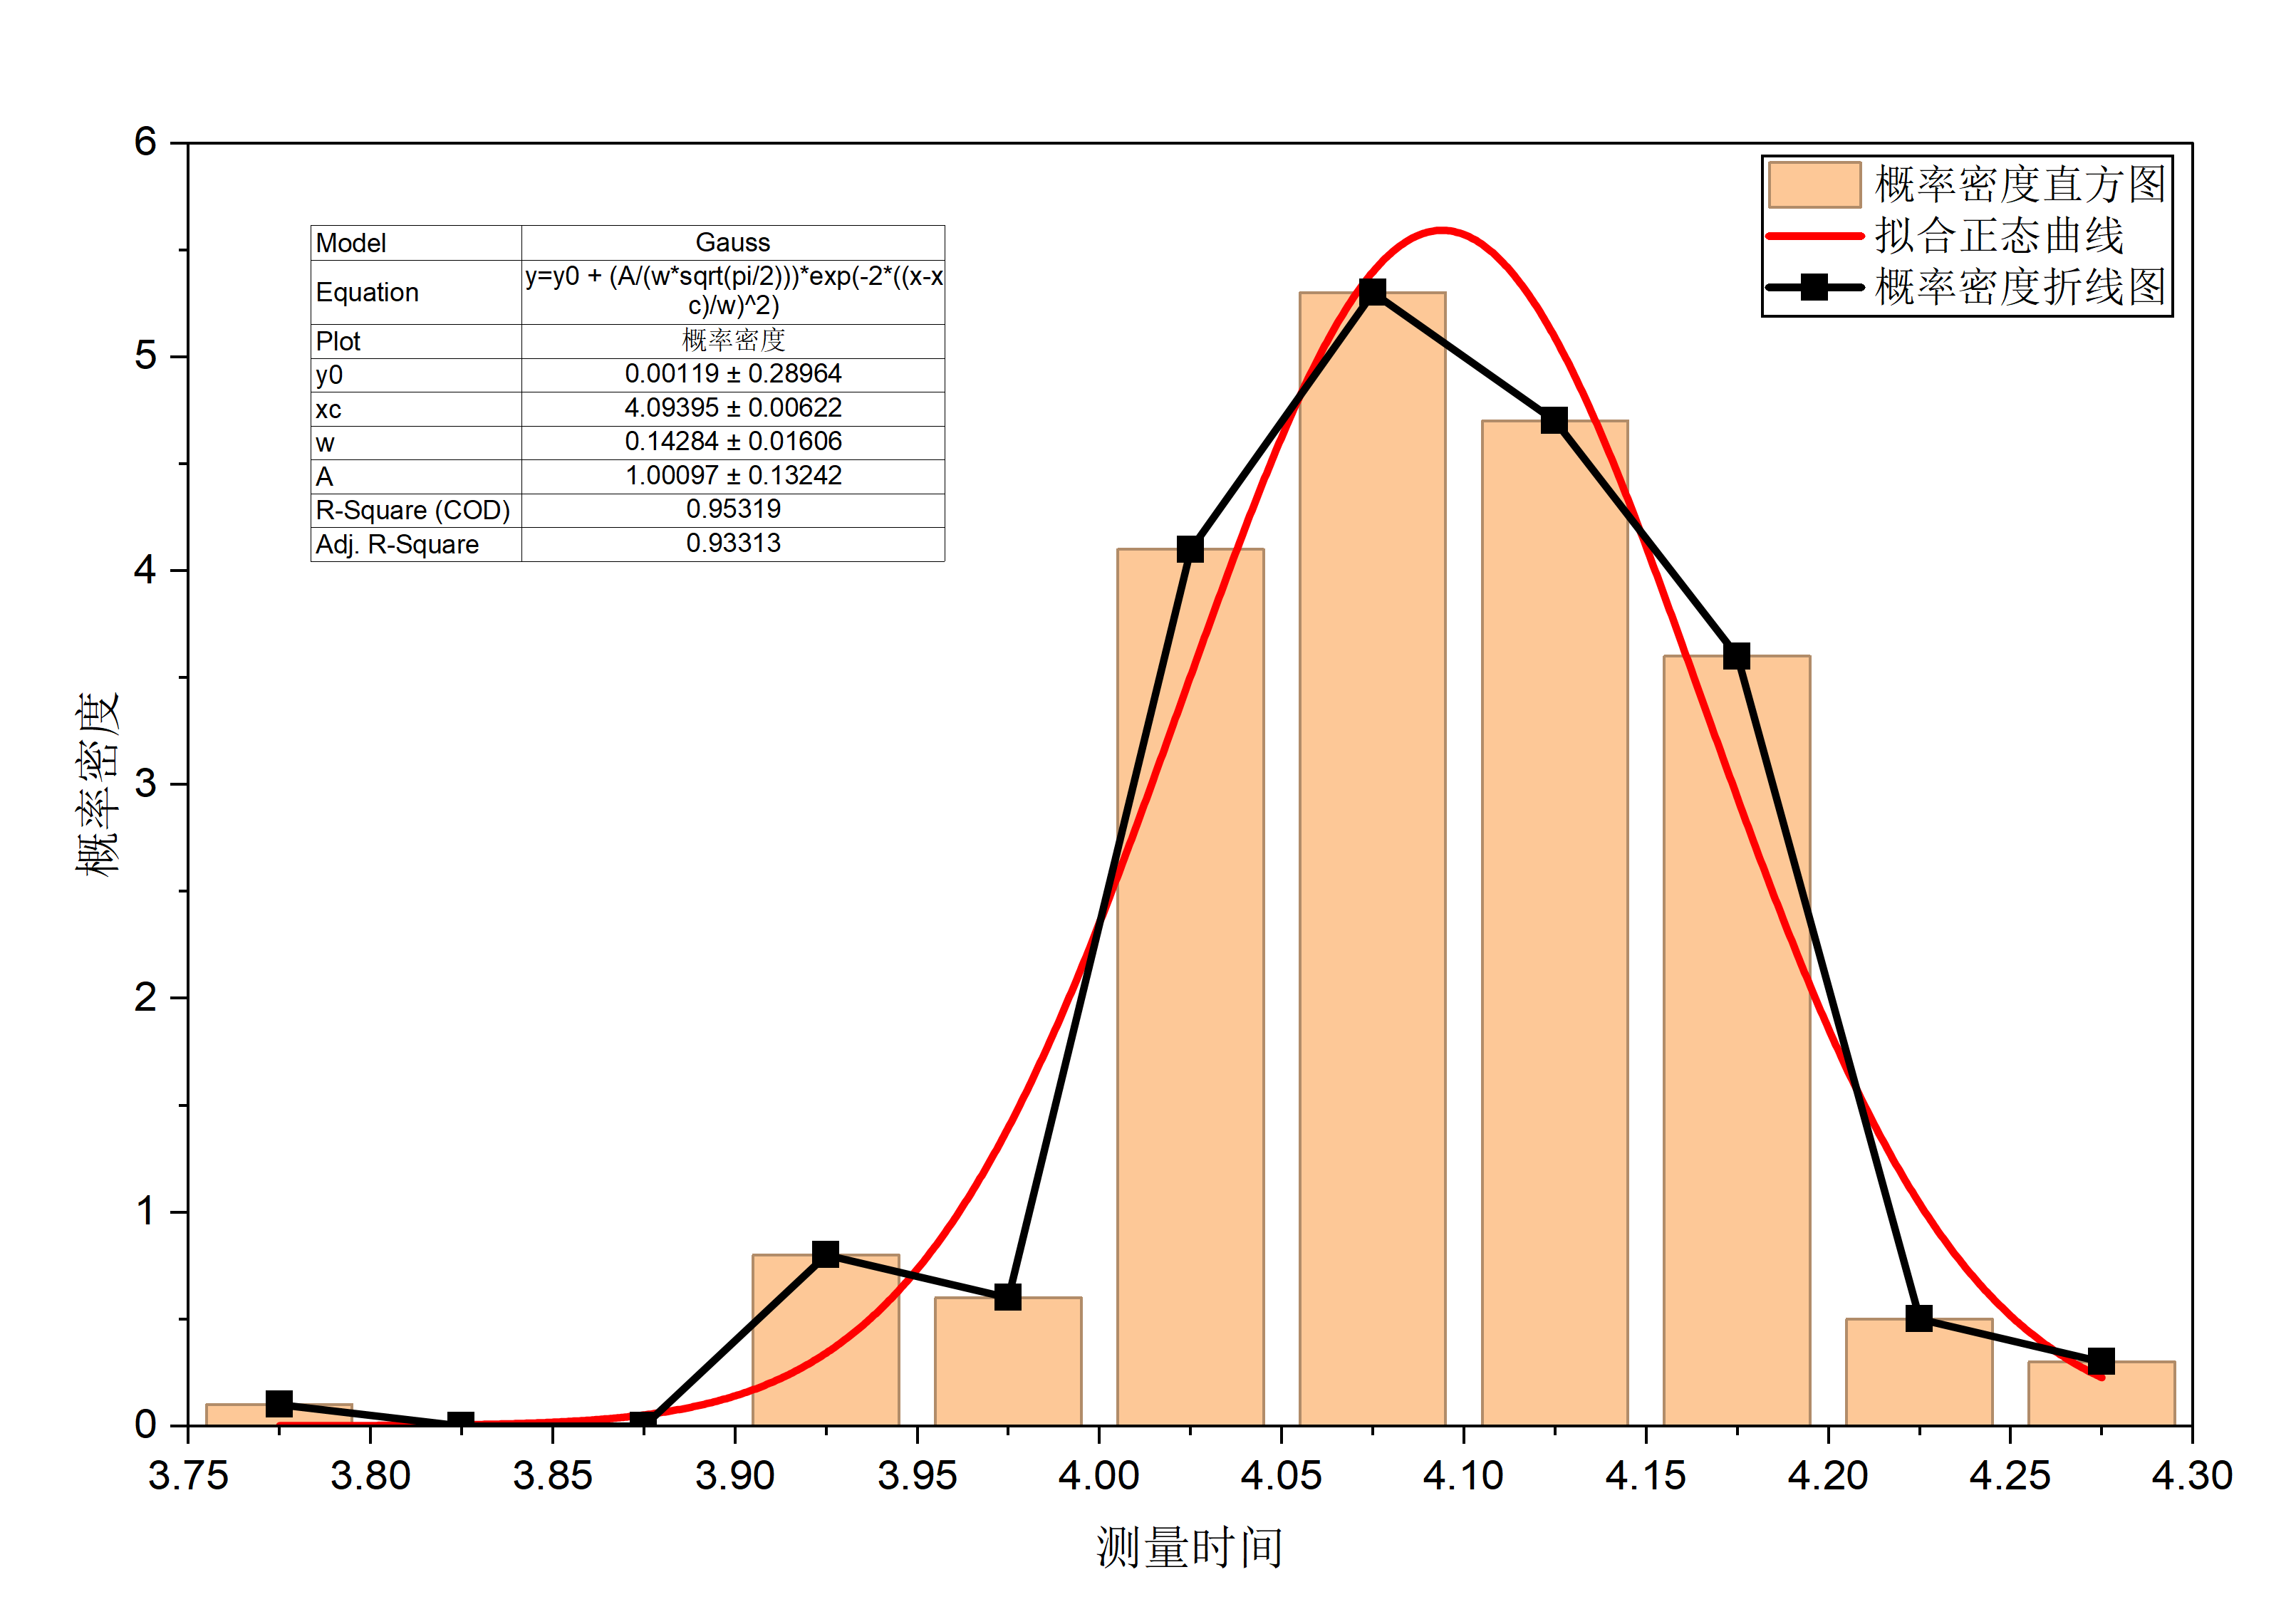
\includegraphics[width=0.8\textwidth]{Graph1.png}
			\caption{测量结果的频率直方图及正态分布拟合曲线}
			\label{fig:histogram}
		\end{figure}
		
		\item 分别统计测量结果出现在各置信区间内的频率和概率，得到：

		\[\ \ \ [\bar{T}-\sigma,\bar{T}+\sigma]=[4.00951, 4.15769], \text{频数:}141, \text{概率:}0.7050\]
		\[[\bar{T}-2\sigma,\bar{T}+2\sigma]= [3.93542, 4.23178], \text{频数:}192, \text{概率:}0.9600\]
		\[[\bar{T}-3\sigma,\bar{T}+3\sigma]= [3.86133, 4.30587], \text{频数:}199, \text{概率:}0.9950\]
		
		与理论值比较：

		\begin{table}[h]
			\centering % 表格居中
			\renewcommand{\arraystretch}{1.3} % 调整行距，1.3 为示例，可根据需要调整
			\begin{tabular}{|c|c|c|c|}
				\hline
				置信区间 & $[\overline{T}-\sigma,\overline{T}+\sigma]$ & $[\overline{T}-2\sigma,\overline{T}+2\sigma]$ & $[\overline{T}-3\sigma,\overline{T}+3\sigma]$ \\ \hline
				概率 & 0.7050 & 0.9600 & 0.9950 \\ \hline
				理论值 & 0.6827 & 0.9545 & 0.9973 \\ \hline
				残差 & 0.0223 & 0.0055 & -0.0023 \\ \hline
			\end{tabular}
			\caption{测量结果与拟合正态分布置信区间的分析} % 添加表格标题
			\label{tab:confidence_intervals} % 添加引用标签
		\end{table}
		
		认为测量结果基本符合正态分布。
		
		\item 不确定度计算
	
		\textbf{A类标准不确定度：}
			$$u_{A}=\frac{\sigma}{\sqrt{n}}=\frac{0.07409}{\sqrt{200}}=0.0052390s$$
		
		\textbf{B类标准不确定度：}
			估计误差来自人开、停秒表的反应时间，取 $\Delta_{\text{估}} = 0.2\mathrm{s}$；
			仪器误差来自秒表，取 $\Delta_{\text{仪}} = 0.01\mathrm{s}$；
			正态分布假设下置信系数 $C=3$。
			则 \[u_B=\dfrac{\sqrt{\Delta_{\text{估}}^2+\Delta_{\text{仪}}^2}}{C}=\frac{\sqrt{(0.2)^{2}+(0.01)^{2}}}{3}=0.0668s\]

		\textbf{不确定度的合成 $(P=0.95)$：}
			正态分布假设下置信因子和 $t$ 因子
			$$t_{0.95}=1.96 \quad k_{0.95}=1.96$$
			则
			$$u_{0.95}=\sqrt{(t_{0.95}u_{A})^{2}+(k_{0.95}u_{B})^{2}}=\sqrt{(1.96\times0.0052390)^{2}+(1.96\times0.0668)^{2}}=0.13133s$$

		\item 测量结果完整表达式
		$$T=\bar{T}\pm u_{0.95} = (4.0836\pm0.13133)s\quad(P=0.95)$$
	
	\end{enumerate}

	\section*{\textbf{{八. 问题思考}}}
	\begin{enumerate}[leftmargin=2em, label=\arabic*.]
		\item 若测量结果偏离正态分布，可能的主要原因包括：
		\begin{itemize}
			\item \textbf{样本量较少：} 本实验重复测量次数较少，随机误差未能充分体现正态分布特性，从而导致观测数据与理论分布存在差异。
			\item \textbf{仪器精度有限：} 本实验使用的秒表精度有限，测量结果可能被取整，导致数据的离散化，从而数据偏离正态分布。
			\item \textbf{实验人员情况：} 本实验受实验人员的操作习惯和反应时间影响较大，影响测量结果的分布形态，如异常数据或偏离中心。
		\end{itemize}
	
		\item 在不考虑系统误差的前提下，多次等精度测量的随机误差分布通常具有以下特征：
		\begin{itemize}
			\item \textbf{正态性：} 根据中心极限定理，随机误差在大量测量中趋近于正态分布，具有集中性、对称性、单峰性等性质。
		\end{itemize}
	\end{enumerate}
	
	\section*{\textbf{{九. 实验结论}}}
	本实验使用秒表重复测量电子节拍器的周期T，并通过统计学方法得到实验测量数据基本符合正态分布，同时计算得到电子节拍器周期，为：
	$$T= (4.0836\pm0.13133)s\quad(P=0.95)$$
	本实验揭示了多次重复等精度测量过程中存在的随机误差的离散性和分布规律。在测量次数充分多时，测量结果的分布趋近于正态分布。
	

\end{document}